% \begin{figure}[ht]
%     \centering
%     \begin{tikzpicture}[scale=1.2]
%       % Draw clusters
%       \draw[dashed, thick] (0,0) circle (1);
%       \draw[dashed, thick] (2.5,0.5) circle (1);
%       \draw[dashed, thick] (1.2,2) circle (1);

%       % Cluster centers
%       \fill[black] (0,0) circle (0.06);
%       \fill[black] (2.5,0.5) circle (0.06);
%       \fill[black] (1.2,2) circle (0.06);

%       % Points for cluster 1
%       \fill[red] (-0.4,0.3) circle (0.08);
%       \fill[blue] (0.5,0.4) circle (0.08);
%       \fill[red] (0.2,-0.6) circle (0.08);
%       \fill[blue] (-0.6,-0.4) circle (0.08);

%       % Points for cluster 2
%       \fill[blue] (2.8,0.2) circle (0.08);
%       \fill[red] (2.2,-0.2) circle (0.08);
%       \fill[red] (2.7,1.2) circle (0.08);
%       \fill[blue] (2,0.8) circle (0.08);

%       % Points for cluster 3
%       \fill[red] (0.9,1.3) circle (0.08);
%       \fill[blue] (1.5,2.3) circle (0.08);
%       \fill[red] (1.1,2.6) circle (0.08);
%       \fill[blue] (0.6,2.1) circle (0.08);

%       % Legend, moved to the right
%       \begin{scope}[shift={(4,1.5)}]
%         \fill[red] (0,1) circle (0.08); \node[right] at (0.2,1) {Group A};
%         \fill[blue] (0,0.7) circle (0.08); \node[right] at (0.2,0.7) {Group B};
%         \draw[dashed, thick] (0,0.4) circle (0.12); \node[right] at (0.2,0.4) {Cluster};
%       \end{scope}

%     \end{tikzpicture}
%     \caption{Illustration of fair clustering with two groups. Each cluster (dashed circle) contains a balanced mix of points from Group A (red) and Group B (blue).}
%     \label{fig:fair-clustering}
% \end{figure}

% \begin{figure}[ht]
% \centering
% \begin{tikzpicture}[scale=1.0, every node/.style={scale=1.0}]
%   % Coordinates for all points (same for both sides)
%   % Top row (Y=3.3 to 3.4)
%   \node[text=blue, scale=0.9]  (A) at (-4,3.4)    {\faFemale};  % in both clusters
%   \node[text=blue, scale=0.9]  (B) at (-3,3.4)    {\faFemale};  % in both clusters
%   \node[text=green!60!black, scale=0.9] (C) at (-2,3.4) {\faMale};     % in fair only
%   \node[text=green!60!black, scale=0.9] (D) at (-1,3.4) {\faMale};     % in fair only

%   % Second row
%   \node[text=blue, scale=0.9]  (E) at (-4.4,2.6)  {\faFemale};        % in unfair only
%   \node[text=green!60!black, scale=0.9] (F) at (-3.5,2.6) {\faMale};  % in both clusters
%   \node[text=blue, scale=0.9]  (G) at (-2.5,2.6)  {\faMale};
%   \node[text=green!60!black, scale=0.9] (H) at (-1.5,2.6) {\faFemale};

%   % Third row
%   \node[text=blue, scale=0.9]  (I) at (-4.2,1.8)  {\faMale};
%   \node[text=green!60!black, scale=0.9] (J) at (-3.2,1.8) {\faFemale};
%   \node[text=blue, scale=0.9]  (K) at (-2.2,1.8)  {\faMale};
%   \node[text=green!60!black, scale=0.9] (L) at (-1.2,1.8) {\faFemale};

%   % --- Left: Unfair cluster (3 blue females + 1 green male: A, B, E, F) ---
%   \draw[thick, blue!70!black] plot [smooth cycle, tension=1] coordinates {
%     (-4.2,3.5)    % A
%     (-2.8,3.6)    % B
%     (-3.5,2.7)    % F
%     (-4.6,2.7)    % E
%   };

%   % Dollar sign (left)
%   \node[text=yellow!80!black, scale=1.7] at (-3.7,3.0) {\$};

%   % Label (left)
%   \node at (-3,3.95) {\large\bfseries Unfair Clustering};

%   % --- Right: All points, mirrored ---
%   % Top row (Y=3.4)
%   \node[text=blue, scale=0.9]  at (2,3.4)   {\faFemale};   % in both clusters
%   \node[text=blue, scale=0.9]  at (3,3.4)   {\faFemale};   % in both clusters
%   \node[text=green!60!black, scale=0.9] at (4,3.4) {\faMale};      % in fair only
%   \node[text=green!60!black, scale=0.9] at (5,3.4) {\faMale};      % in fair only

%   % Second row
%   \node[text=blue, scale=0.9]  at (1.6,2.6)  {\faFemale};         % in unfair only
%   \node[text=green!60!black, scale=0.9] at (2.5,2.6) {\faMale};   % in both clusters
%   \node[text=blue, scale=0.9]  at (3.5,2.6)  {\faMale};
%   \node[text=green!60!black, scale=0.9] at (4.5,2.6) {\faFemale};

%   % Third row
%   \node[text=blue, scale=0.9]  at (1.8,1.8)  {\faMale};
%   \node[text=green!60!black, scale=0.9] at (2.8,1.8) {\faFemale};
%   \node[text=blue, scale=0.9]  at (3.8,1.8)  {\faMale};
%   \node[text=green!60!black, scale=0.9] at (4.8,1.8) {\faFemale};

%   % --- Right: Fair cluster (2 blue females + 2 green males: A, B, C, D mirrored) ---
%   \draw[thick, blue!70!black] plot [smooth cycle, tension=1] coordinates {
%     (1.8,3.5)    % A
%     (3.2,3.6)    % B
%     (4.8,3.5)    % D
%     (3.7,2.7)    % C (was F in left, but use top left 2 blue, top left 2 green)
%   };

%   % Dollar sign (right)
%   \node[text=yellow!80!black, scale=1.7] at (3.4,3.0) {\$};

%   % Label (right)
%   \node at (3.5,3.95) {\large\bfseries Fair Clustering};

%   % -- Legend (right) --
%   \begin{scope}[shift={(6,2.8)}]
%     \node[text=blue, scale=0.9] (L1) at (0,0.8) {\faFemale};
%     \node[right] at (0.3,0.8) {Group 1};
%     \node[text=green!60!black, scale=0.9] (L2) at (0,0.4) {\faMale};
%     \node[right] at (0.3,0.4) {Group 2};
%     \node[text=yellow!80!black, scale=0.9] at (0,0) {\$};
%     \node[right] at (0.3,0) {Resource};
%   \end{scope}
% \end{tikzpicture}
% \caption{
% \textbf{Left:} Unfair clustering, with a cluster containing 3 blue females and 1 green male.
% \textbf{Right:} Fair clustering, with a cluster containing 2 blue females and 2 green males. The same set of individuals are clustered differently to illustrate the effect of fairness constraints. Icons indicate individuals from two groups (e.g., by gender or demographic feature).
% }
% \label{fig:fair-unfair-clustering-same-layout}
% \end{figure}


\begin{figure}[ht]
    \centering
    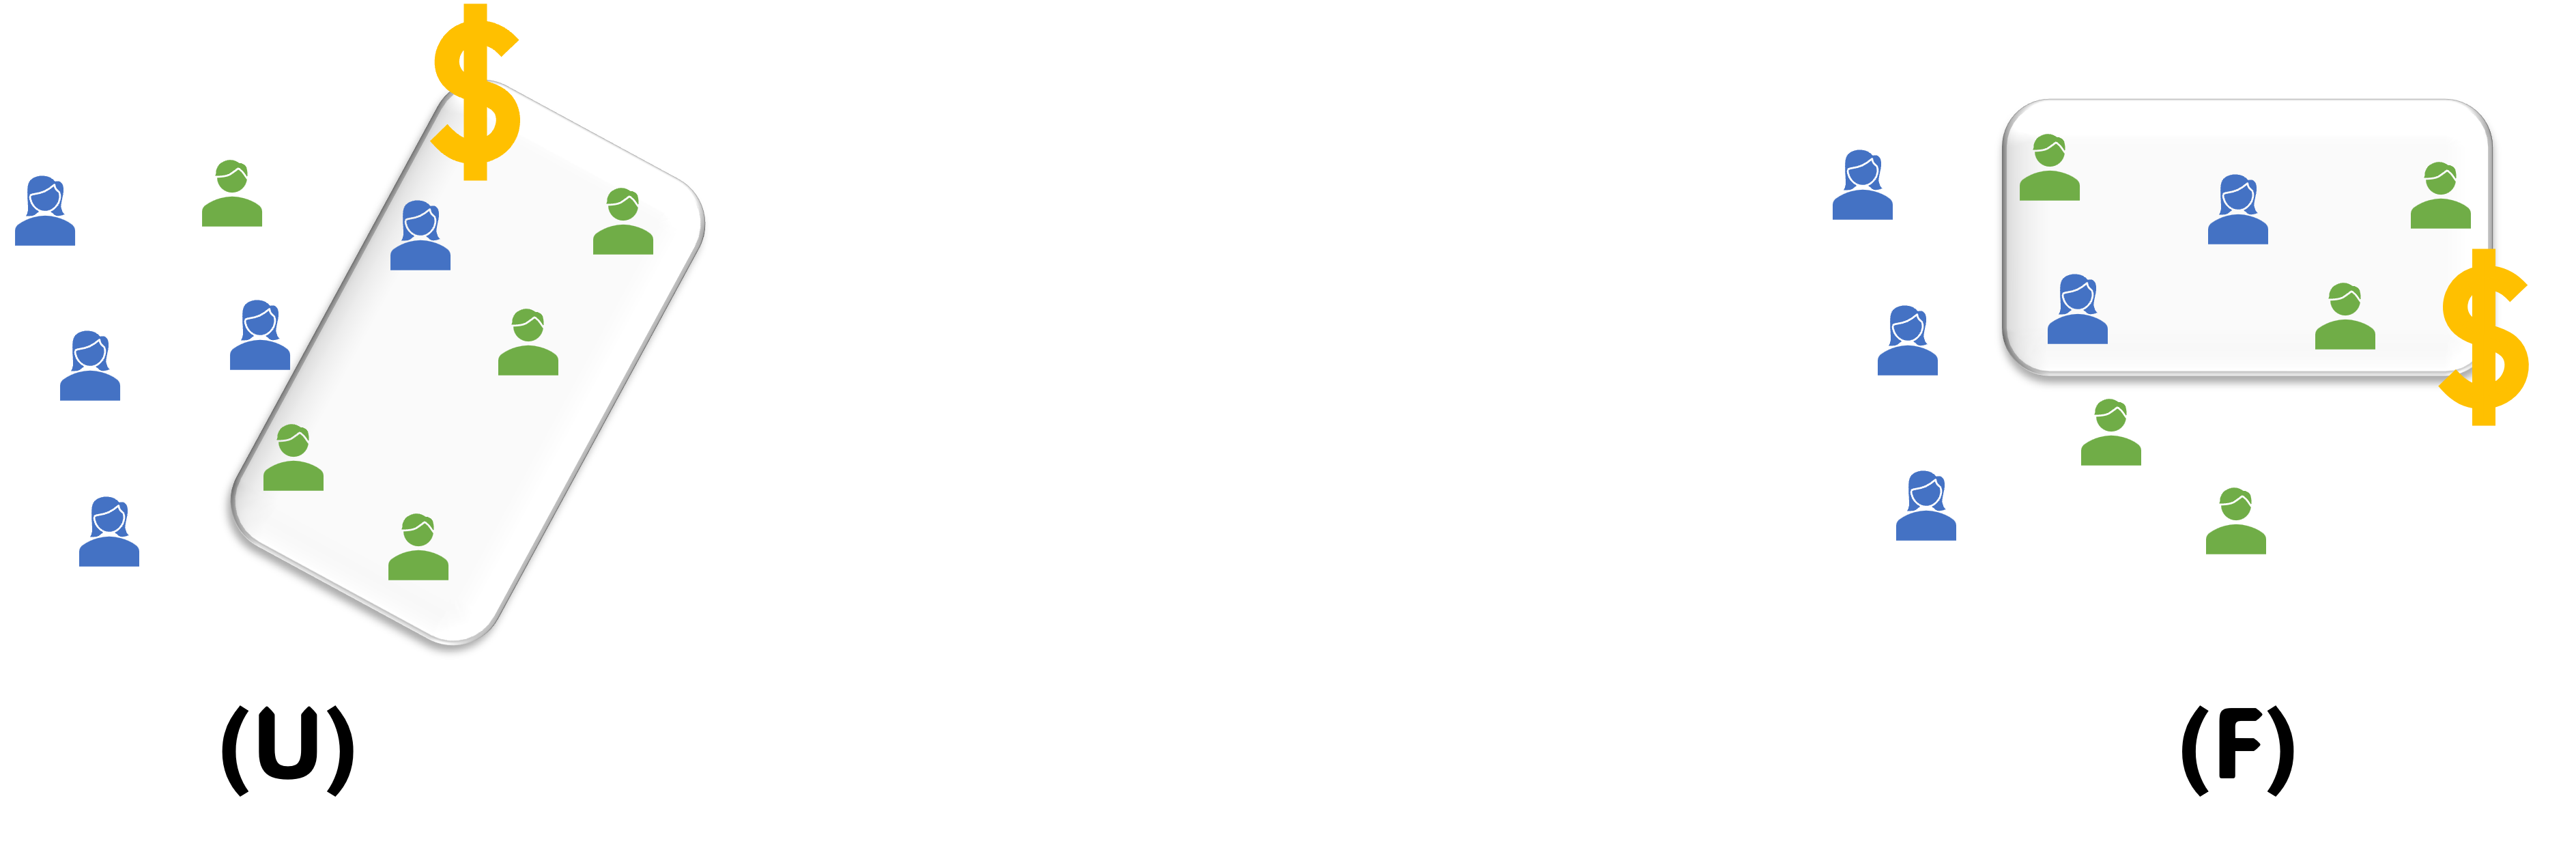
\includegraphics[width=0.75\textwidth]{images/bal_rep_cluster.png}
    \caption{
        \textbf{Left $(\mathsf{U})$:} An unbalanced clustering, where the selected cluster is dominated by individuals from one group (green), with only a single member from the other group, resulting in unequal representation in the advantaged cluster. \textbf{Right (F):} A more balanced clustering.
    }
    \label{fig:bal_rep_clustering}
\end{figure}
